%%%%%%%%%%%%%%%%%%%%%%%%%%%%%%%%%%%%%%%%%%{{{
% Structured General Purpose Assignment
% LaTeX Template
%
% This template has been downloaded from:
% http://www.latextemplates.com
%
% Original author:
% Ted Pavlic (http://www.tedpavlic.com)
%
% Note:
% The \lipsum[#] commands throughout this template generate dummy text
% to fill the template out. These commands should all be removed when 
% writing assignment content.
%
%%%%%%%%%%%%%%%%%%%%%%%%%%%%%%%%%%%%%%%%%

%----------------------------------------------------------------------------------------
%	PACKAGES AND OTHER DOCUMENT CONFIGURATIONS
%----------------------------------------------------------------------------------------

\documentclass[12pt,a4paper]{article}

\usepackage{fancyhdr} % Required for custom headers
\usepackage[utf8]{inputenc}
\usepackage[french]{babel}
\usepackage{hyperref}
\usepackage{hyperref}
\usepackage{float}
\usepackage{lastpage} % Required to determine the last page for the footer
\usepackage{extramarks} % Required for headers and footers
\usepackage{graphicx} % Required to insert images
\usepackage{lipsum} % Used for inserting dummy 'Lorem ipsum' text into the template

% Margins
\topmargin=-0.45in
\evensidemargin=0in
\oddsidemargin=0in
\textwidth=6.5in
\textheight=9.0in
\headsep=0.25in 

\linespread{1.1} % Line spacing

% Set up the header and footer
\pagestyle{fancy}
\lhead{\hmwkAuthorName \ \hmwkTitle} % Top left header
\rhead{\firstxmark} % Top right header
\lfoot{\lastxmark} % Bottom left footer
\cfoot{} % Bottom center footer
\rfoot{Page\ \thepage\ de\ \pageref{LastPage}} % Bottom right footer
\renewcommand\headrulewidth{0.4pt} % Size of the header rule

\renewcommand\footrulewidth{0.4pt} % Size of the footer rule

\setlength\parindent{0pt} % Removes all indentation from paragraphs

%----------------------------------------------------------------------------------------
%	DOCUMENT STRUCTURE COMMANDS
%	Skip this unless you know what you're doing
%----------------------------------------------------------------------------------------

% Header and footer for when a page split occurs within a problem environment
\newcommand{\enterProblemHeader}[1]{
\nobreak\extramarks{#1}{#1 continue \ldots}\nobreak
\nobreak\extramarks{#1 (suite)}{#1 continue \ldots}\nobreak
}

% Header and footer for when a page split occurs between problem environments
\newcommand{\exitProblemHeader}[1]{
\nobreak\extramarks{#1 (continued)}{#1 continued on next page\ldots}\nobreak
\nobreak\extramarks{#1}{}\nobreak
}

\setcounter{secnumdepth}{0} % Removes default section numbers
\newcounter{homeworkProblemCounter} % Creates a counter to keep track of the number of problems
\newcounter{homeworkQuestionCounter} % Creates a counter to keep track of the number of problems

\newcommand{\homeworkProblemName}{}
\newenvironment{homeworkProblem}[1][Problem \arabic{homeworkProblemCounter}]{ % Makes a new environment called homeworkProblem which takes 1 argument (custom name) but the default is "Problem #"
\stepcounter{homeworkProblemCounter} % Increase counter for number of problems
\renewcommand{\homeworkProblemName}{#1} % Assign \homeworkProblemName the name of the problem
\section{\homeworkProblemName} % Make a section in the document with the custom problem count
\enterProblemHeader{\homeworkProblemName} % Header and footer within the environment
}{
\exitProblemHeader{\homeworkProblemName} % Header and footer after the environment
\setcounter{homeworkQuestionCounter}{0} % Removes default section numbers
}

\newcommand{\problemAnswer}[1]{ % Defines the problem answer command with the content as the only argument
\noindent\framebox[\columnwidth][c]{\begin{minipage}{0.98\columnwidth}#1\end{minipage}} % Makes the box around the problem answer and puts the content inside
}

\newcommand{\homeworkSectionName}{}
\newenvironment{homeworkSection}[1]{ % New environment for sections within homework problems, takes 1 argument - the name of the section
\stepcounter{homeworkQuestionCounter} % Increase counter for number of problems
\renewcommand{\homeworkSectionName}{\arabic{homeworkProblemCounter} . \arabic{homeworkQuestionCounter} #1} % Assign \homeworkSectionName to the name of the section from the environment argument
\subsection{\homeworkSectionName} % Make a subsection with the custom name of the subsection
\enterProblemHeader{\homeworkProblemName\ [\homeworkSectionName]} % Header and footer within the environment
}{
\enterProblemHeader{\homeworkProblemName} % Header and footer after the environment
}
   
%----------------------------------------------------------------------------------------
%	NAME AND CLASS SECTION
%----------------------------------------------------------------------------------------

\newcommand{\hmwkTitle}{TP1} % Assignment title
\newcommand{\hmwkDueDate}{Mardi\ 2 Février\ 2016} % Due date
\newcommand{\hmwkClass}{INF6422} % Course/class
\newcommand{\hmwkClassTime}{12h} % Class/lecture time
\newcommand{\hmwkClassInstructor}{François Labrèche} % Teacher/lecturer
\newcommand{\hmwkAuthorName}{Philippe Troclet (1815208) et Alexandre Mao (1813566)} % Your name

%----------------------------------------------------------------------------------------
%	TITLE PAGE
%----------------------------------------------------------------------------------------

\title{
\vspace{2in}
\textmd{\textbf{\hmwkClass:\ \hmwkTitle}}\\
\normalsize\vspace{0.1in}\small{pour\ le\ \hmwkDueDate}\\
\vspace{3in}
}

\author{\textbf{\hmwkAuthorName}}
\date{} % Insert date here if you want it to appear below your name

%----------------------------------------------------------------------------------------

\begin{document}

\maketitle

%----------------------------------------------------------------------------------------
%	TABLE OF CONTENTS
%----------------------------------------------------------------------------------------

%\setcounter{tocdepth}{1} % Uncomment this line if you don't want subsections listed in the ToC

\newpage
\tableofcontents
\newpage%}}}

%----------------------------------------------------------------------------------------
%	Première partie
%----------------------------------------------------------------------------------------

\begin{homeworkProblem}[\arabic{homeworkProblemCounter} Modèle déterministe] % Custom section title

\begin{homeworkSection}{Choix d'un modèle comportemental} % Section within problem
    % j'ai mis en commentaires le cadre autour de la réopnse, je trouvais que c'étais un peu too much xD, mais si tu eux le
    % remettre, fais toi plaisir.
%\problemAnswer{ % Answer
En regardant tout d'abord les 3 modèles, nous pouvons constater les caractéristiques suivantes pour chaque modèle :
\begin{itemize}
    \item Modèle SI : Le modèle SI (avec S représentant le nombre de machines saines et I le nombre de machines infectées) représente l'évolution d'une épidémie ,dans une population à une ou plusieurs machines infectées, de la contagion auprès du reste de la population en ne prenant en compte que le facteur que les machines infectées vont infecter les machines saines.
    \item Modèle SIS : Le modèle SIS (avec S représentant le nombre de machines saines et I le nombre de machines infectées) représente l'évolution d'une épidémie dans une population à un ou plusieurs facteurs patogènes. On considère dans ce cas que le facteur pathogène n'est que temporaire et se guérit au bout d'un laps de temps donné. Une machine infectée aura le pouvoir de "se guérir" toute seule pour repasser dans l'état sain.
    \item Modèle SIR : Le modèles SIR (avec S représentant le nombre de machines saines, I le nombre de machines infectées et R le nombre de machines qui ont été guéries et immunisées) représente l'évolution d'une épidémie dans une population où on va introduire auprès de la population un vacin contre le ou les facteur(s) pathogène(s). Une machine infectée pourra alors recevoir le vaccin ou l'antidote et se retrouver immunisée contre l'agent pathogène.
\end{itemize}

En nous basant sur l'article "Optimising Networks Against Malware", le modèle comportemental qui s'appliquerait serait le modèle
SI. En effet, dans l'article, les auteurs s'intéressent à l'évolution d'un ver(agent pathogène) dans un réseau avec un nombre
défini de machines (population étudiée). Les machines ne possédant pas de système immunitaire qui pourrait être représenté par un
anti-virus, ou un logiciel interne qui scannerait le système pour rechercher et éliminer des facteurs et externes, nous ne pouvons
pas être dans le cas SIS. Et il n'y a pas de référence dans l'article à des mises à jours du système ou d'un anti-virus éventuel,
nous pouvons conclure qu'il n'y a pas d'injection de remèdes contre les vers et que les machines n'ont nullement été guéries et
immunisées contre cet agent pathogène et donc que nous ne pouvons pas nous trouver dans le cas du modèle SIR. Ainsi comme cet
article étudie simplement l'évolution de l'infection d'un ensemble de machines dans différentes configurations données, nous
pouvons donc penser que c'est bien le modèle SI qui s'appliquerait. Notons que cette conclusion est légitime de part l'absence de
guérison (pas d'anti-virus) ainsi que l'impossibilité pour une machine de se déconnecter, ou de quitter le réseau. Pour connaître
de façon plus précise les hypothèses utilisées dans le cadre de l'article, on pourra se reporter au premier paragraphe de la partie
2.3 du dit article, intitulé : \it{"Markov process Model"}.
%}
\end{homeworkSection}

%--------------------------------------------

\begin{homeworkSection}{Identification des équations différentielles} % Section within problem
    Dans la question précédente, nous avions déterminé qu'un modèle compartimental de type SI s'appliquait à l'étude de la
propagation des logiciels malveillants. Sachant qu'un ordinateur peut être sain ou infecté, et uniquement l'un de
ces deux états, on a la première relation:
\[
    S + I = N
\]
Où $N$ est la taille de la population et $S$ la taille de la population saine. Tandis que $I$ est la taille population infectée. Si de
plus, on note $\lambda$ le nombre de contacts par machine par unité de temps, On a alors que \( \lambda \cdot I \) représente le
nombre de machine qui ont été atteintes par une machine infecté entre deux unités de temps. Sachant que \( \frac{S}{N} \) est la
proportion de machines saines à l'instant courant, on peut approximer le nombre de machines nouvellement infectées entre deux pas
de temps par \( \lambda \cdot I \cdot \frac{S}{N} \). Ce qui nous donne l'équation différentielle suivante:
\[
    \frac{dI(t)}{dt} = \lambda \cdot I(t) \cdot \frac{S(t)}{N}
\]
On peut alors remplacer $S(t)$ par $N - I(t)$, et on obtient:
\[
    \frac{dI(t)}{dt} = \lambda \cdot I(t) \cdot \frac{N-I(t)}{N}
\]
De part la relation entre $S$ et $I$, on a:
\[
    \frac{dS(t)}{dt} + \frac{dI(t)}{dt} = 0
\]
De ce fait, \( \frac{dS(t)}{dt} = -\lambda \cdot (N-S(t)) \cdot \frac{S(t)}{N} \).
\end{homeworkSection}

%--------------------------------------------

\end{homeworkProblem}

%----------------------------------------------------------------------------------------
%	PROBLEM 3
%----------------------------------------------------------------------------------------

\begin{homeworkProblem}[\arabic{homeworkProblemCounter} Simulation numériques] % Roman numerals

%--------------------------------------------

\begin{homeworkSection}{Etude de I et S en fonction du temps} % Using the problem name elsewhere
\begin{figure}[H]
    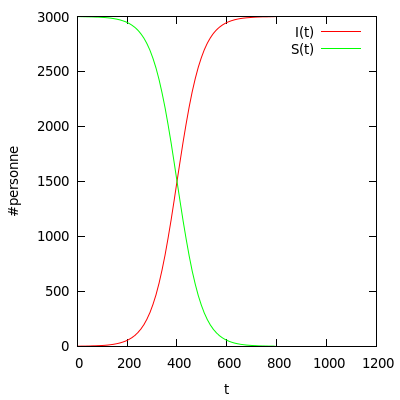
\includegraphics{Images/plotting_Q3_1.png}
    \caption{évolution de la population en fonction du temps}
    \label{fig:Q3.1}
\end{figure}
\end{homeworkSection}

%--------------------------------------------

\begin{homeworkSection}{Etude de l'influence du paramètre $\lambda$}
\begin{figure}[H]
    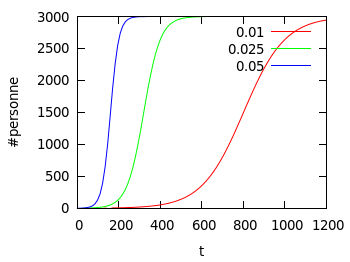
\includegraphics{Images/plotting_Q3_2.png}
    \caption{influence du paramètre $\lambda$}
    \label{fig:Q3.2}
\end{figure}
\end{homeworkSection}

%--------------------------------------------

\end{homeworkProblem}

%----------------------------------------------------------------------------------------
%	PROBLEM 4
%----------------------------------------------------------------------------------------

\begin{homeworkProblem}[\arabic{homeworkProblemCounter} Modèle stochastique] % Roman numerals
\problemAnswer{ % Answer
\lipsum[10]
}
\end{homeworkProblem}

%----------------------------------------------------------------------------------------

\end{document}
